\documentclass[10pt,a4paper]{article}

\usepackage[utf8]{inputenc}
\usepackage{amsmath}
\usepackage{amsfonts}
\usepackage{amssymb}
\usepackage{tikz}
\usepackage{pgf}
\usepackage{pgfplots}
\usepackage{hyperref}
\usepackage{comment}
\usepackage{algorithm}
\usepackage[noend]{algpseudocode}
\usepackage{parskip}
\usepackage{listings}
\usepackage{xcolor}

\pgfplotsset{compat=1.3}
\title{Implementation and evaluation of the small progress measures algorithm}

\author{Olav Bunte (0803961, o.bunte@student.tue.nl),\\
Maurice Laveaux (0813568, m.laveaux@student.tue.nl),\\
Ziad Ben Snaiba (0748095, z.b.snaiba@student.tue.nl)}

\date{\today}

\begin{document}
\maketitle

\section{Introduction}
This report elaborates on our work and findings of assignment two. The goal of this assignment is to implement and evaluate the small progress measures algorithm as described in \cite{spmpaper}. First we will address the design and implementation of the algorithm in section \ref{design}, along with alternative lifting strategies to make the algorithm more efficient. Then in section \ref{eval} we will show the performance of each lifting strategy using self-made and provided parity games. Lastly, we will reach a conclusion in section \ref{conc}.

\section{Design and implementation}\label{design}
In this section the design and implementation of our small progress measures algorithm is given, which we have programmed using C++. First we will show the data structure
used to store a parity game. Then we elaborate on the design of the small progress measures algorithm itself. Lastly we will show the lifting orders implemented and explain their advantages.

\subsection{Parity Game}

\subsection{Small progress measures}
For this algorithm we needed another data structure, namely for progress measures. For this we have chosen to define \verb|Measure| as a vector of $p$ integers where $p$ is the maximum priority of the parity game plus one. The special progress measure \verb|TOP| is a vector of only one element, namely the integer 1. The set of possible progress measures for a parity game is also represented by a \verb|Measure|, holding the maximum value for each uneven element.
\\\\
The small progress measures algorithm is split up in five separate methods:
\begin{itemize}
\item \verb|getProgressMeasures|: gets the set of all progress measures possible for a given parity game.
\item \verb|lexicoGreaterThan|: determines whether a \verb|Measure| is lexicographically greater than another \verb|Measure|. Can be strict or non-strict and can be tested up to a certain element.
\item \verb|prog|: computes the value of \textit{Prog} as defined in the slides and in \cite{spmpaper} given a vertex and one of its successors.
\item \verb|lift|: lifts a vertex as defined in the slides and in \cite{spmpaper}.
\item \verb|solveParityGame|: the main algorithm itself.
\end{itemize}
See figures \ref{alg:getProgMeas}, \ref{alg:lexico}, \ref{alg:prog}, \ref{alg:lift} and \ref{alg:solve} for the pseudo code of above methods respectively.
\\\\
From the definition of a measure, we know that each even element of the measure is always zero. This is used to speed up the creation and comparison of these measures by iterating only over all uneven elements of the measure. Note that because of this we need an extra check to be able to compare to \verb|TOP|. The application of this can be seen in the pseudo code in figures \ref{alg:getProgMeas}, \ref{alg:lexico} and \ref{alg:prog}.

\subsection{Lifting orders}

\subsubsection{Input}
This lifting order simply iterates over the vertices in the order of the input, starting by 0 and incrementing by one every vertex. There is no real advantage or rationale behind this order, except that it is deterministic and it is easy to compute.

\subsubsection{Random}
This lifting order, as the name suggests, uses a random ordering of all vertices. This ordering is set at the start of the execution of the algorithm.\\
The randomness causes multiple executions of the algorithm to be non-deterministic, giving different execution times every execution. This can, depending on the created order, either be an advantage or a disadvantage. It can happen that in one execution the order is very efficient and in another execution it is very inefficient.

\subsubsection{In degree}\label{indegree}
This lifting order is based on the fact that the \verb|prog| method takes the measure of a successor vertex and either tries to increase it or copy it. In this order all vertices are descendingly ordered on their in degree (the amount of incoming edges). Since \verb|prog| uses successors to create a measure, more vertices will have profit in the same iteration over the order when first lifting a vertex with a higher in degree than when first lifting a vertex with a lower in degree.


This order works well with parity games with a big varying in degree for the nodes. Especially parity games with a star-like form, where many vertices point to one vertex, have profit form this order. In such a case the vertex in the center of the star will be lifted first. Afterwards the vertices on the points of the star will be lifted, profiting form the lifted center vertex.

\subsubsection{Breadth first search}
% Explanation
Like the previous order, this lifting order is based on the fact that the \verb|prog| method takes the measure of a successor vertex and either tries to increase it or copy it. When this successor vertex was already lifted beforehand the resulting measure for the lifted vertex will be even higher. So a breadth first search that places a vertex before its predecessors can possibly increase performance. It is not always possible to get all vertices starting from a single position, thus when the order is not complete the next smallest vertex is selected and another breadth first search is conducted. The implementation code is included in the appendix under \ref{appendix:bfs}.

% Optimal example
An example where this order is more efficient then the others is a single cycle where every vertex has a neighbour as successor. The input order doesn't have to follow the cycle reversed and the in-degree is the same for all vertices. So in this case the breadth first search will put the vertices in reversed order and the measures will be lifted faster.\\
Note that this order is not necessarily better in the example parity game given for the in degree. For example, if the center vertex of the star is the last vertex in the input, the order is actually quite bad. This gave us the idea of creating a fifth lifting order.

\subsubsection{Breadth first search with in degree order}
This lifting order combines the advantages and rationale of the two orders above. It first creates the in degree order as described in section \ref{indegree}. Then it uses the first vertex in this order to start the first breadth first search. When the search cannot go any further but there are vertices left, it will start a new search from the first vertex in the in degree order that hasn't been found yet.

\section{Evaluation}\label{eval}

\subsection{Self-made parity games}

\begin{enumerate}[Game01]
	\item Even wins \{0, 1\} and odd wins \{2, 3, 4, 5, 6\}
\end{enumerate}

\subsection{Dining Philosophers}

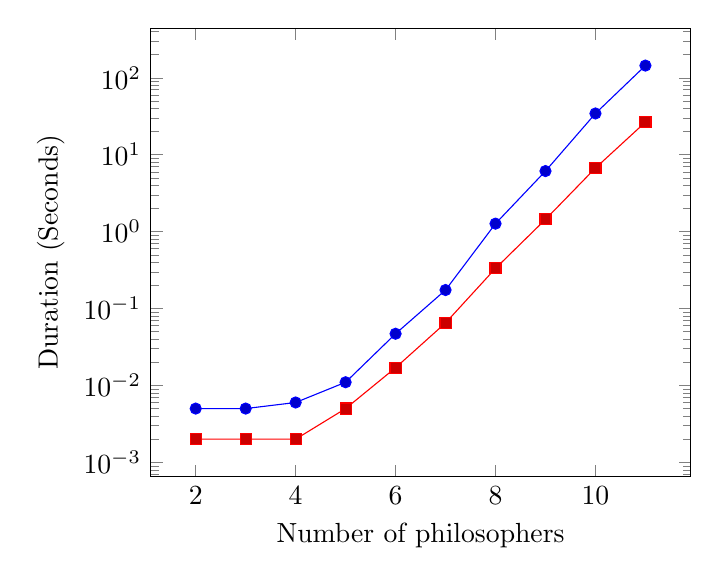
\begin{tikzpicture}
  	\begin{axis}[ 
    	xlabel={Number of philosophers},
    	ylabel={Duration (Seconds)},
    	ymode=log,
        log basis y={10}
  	] 
    \addplot+ [color=blue] coordinates {(2, 0.005) (3, 0.005) (4, 0.006) (5, 0.011) (6, 0.047) (7, 0.174) (8, 1.270) (9, 6.131) (10, 34.391) (11, 144.252)}; 
    
    \addplot+ [color=red] coordinates {(2, 0.002) (3, 0.002) (4, 0.002) (5, 0.005) (6, 0.017) (7, 0.065) (8, 0.333) (9, 1.442) (10, 6.716) (11, 26.529)}; 
  	\end{axis}
\end{tikzpicture}

\subsection{Elevator}


\section{Conclusion}\label{conc}


\begin{thebibliography}{9}
\bibitem{spmpaper} M. Jurdzi\'{n}ski: Small Progress Measures for Solving Parity Games, March 2000
\end{thebibliography}


\newpage
\appendix

\section{Breadth first order}\label{appendix:bfs}

\begin{verbatim}
// Create the order and coloring vectors.
order = std::vector<Vertex>(parityGame.getNumberOfVertices(), -1);
std::vector<int> graphColoring(parityGame.getNumberOfVertices());

// The queue for to be handled vertices.
std::queue<Vertex> workQueue;

// The current order being search and vertex beind handled.
int ordering = 0;
Vertex currentVertex = 0;

while (ordering != parityGame.getNumberOfVertices()) {
	workQueue.push(currentVertex); // Add the first vertex.

    while (!workQueue.empty()) {
    	// Pop the first element.
        Vertex current = workQueue.front(); workQueue.pop();

        if (graphColoring[current] == 0) {
        	// If the color is not yet set .
            for (auto& incomingVertex : parityGame.getIncomingVertices(current)) {
            	workQueue.push(incomingVertex);
            }

            // Color the current vertex.
            graphColoring[current] = 1;
            order[ordering++] = current;
        }
    }

    // Select the smallest vertex not yet put into ordering.
    for (Vertex current = 0; current < graphColoring.size(); ++current) {
    	if (graphColoring[current] == 0) {
        	currentVertex = current;
            break;
        }
    }
}
\end{verbatim}






\end{document}